\documentclass[11pt]{article}
\usepackage[margin=1in]{geometry}
\usepackage{graphicx}
\usepackage{booktabs}
\usepackage{amsmath}
\usepackage{amssymb}
\usepackage{hyperref}
\usepackage{float}
\usepackage{subcaption}
\usepackage{xcolor}
\usepackage{longtable}
\usepackage{array}
\usepackage{placeins}
\usepackage{pdflscape}
\usepackage{adjustbox}
\title{Mapper/TDA Report for Imputed PSCompPars}
\date{}
\begin{document}
\maketitle
Se construyeron grafos Mapper sobre el catalogo PSCompPars completado. La imputacion principal es iterative. Los valores se trazan como observed, physically derived o imputed. El objetivo es analisis exploratorio topologico, no prueba final de clases planetarias.

\section{Introduction}
No interpretamos Mapper como prueba directa de la topologia real de los exoplanetas. Interpretamos los grafos como estructuras inducidas por una matriz completada con trazabilidad explicita. Las regiones mas confiables son aquellas con baja fraccion de imputacion, estabilidad bajo cambios de lens, imputacion y parametros, y coherencia con variables fisicas planetarias.

\section{Data and Imputation}
El dataset usa siete variables principales: pl_rade, pl_bmasse, pl_dens, pl_orbper, pl_orbsmax, pl_insol y pl_eqt. Mapper usa una matriz transformada y escalada, mientras que la interpretacion usa el CSV fisico con unidades y banderas de procedencia. Se distinguen explicitamente observed, physically_derived e imputed. Las derivaciones fisicas usadas incluyen $pl\_dens = 5.514 \cdot pl\_bmasse / pl\_rade^3$ y $pl\_orbsmax = (st\_mass \cdot (pl\_orbper / 365.25)^2)^{1/3}$. pl\_dens es mayoritariamente derivada desde pl\_bmasse y pl\_rade; por tanto, no debe tratarse como observacion independiente cuando se usa junto con masa y radio.

\section{Mapper Methodology}
Sea $X = \{x_1, \ldots, x_n\} \subset \mathbb{R}^p$. Sea $f: X \to \mathbb{R}^d$ un lens y $\mathcal{U}=\{U_\alpha\}$ una cubierta del espacio de lentes. Para cada $U_\alpha$ se clusteriza $f^{-1}(U_\alpha)$ y se construye un grafo donde los nodos son clusters locales y las aristas representan interseccion no vacia de miembros. Usamos $\beta_1 = E - V + C$ con $E$ aristas, $V$ nodos y $C=\beta_0$ componentes conexas. La configuracion base usa n\_cubes=10, overlap=0.35, DBSCAN, min\_samples=4, eps\_percentile=90 y random\_state=42.

\section{Mapper Results}
Los resultados principales se resumen en las figuras estaticas globales y en los grafos `joint_no_density` y `joint` con lens pca2. La configuracion con mayor complejidad combinada fue `orbital_pca2_cubes10_overlap0p35`, con 124 nodos y beta_1=96. Esto no prueba clases planetarias finales: resume estructura inducida por una matriz completada y auditada. \begin{figure}[H]\centering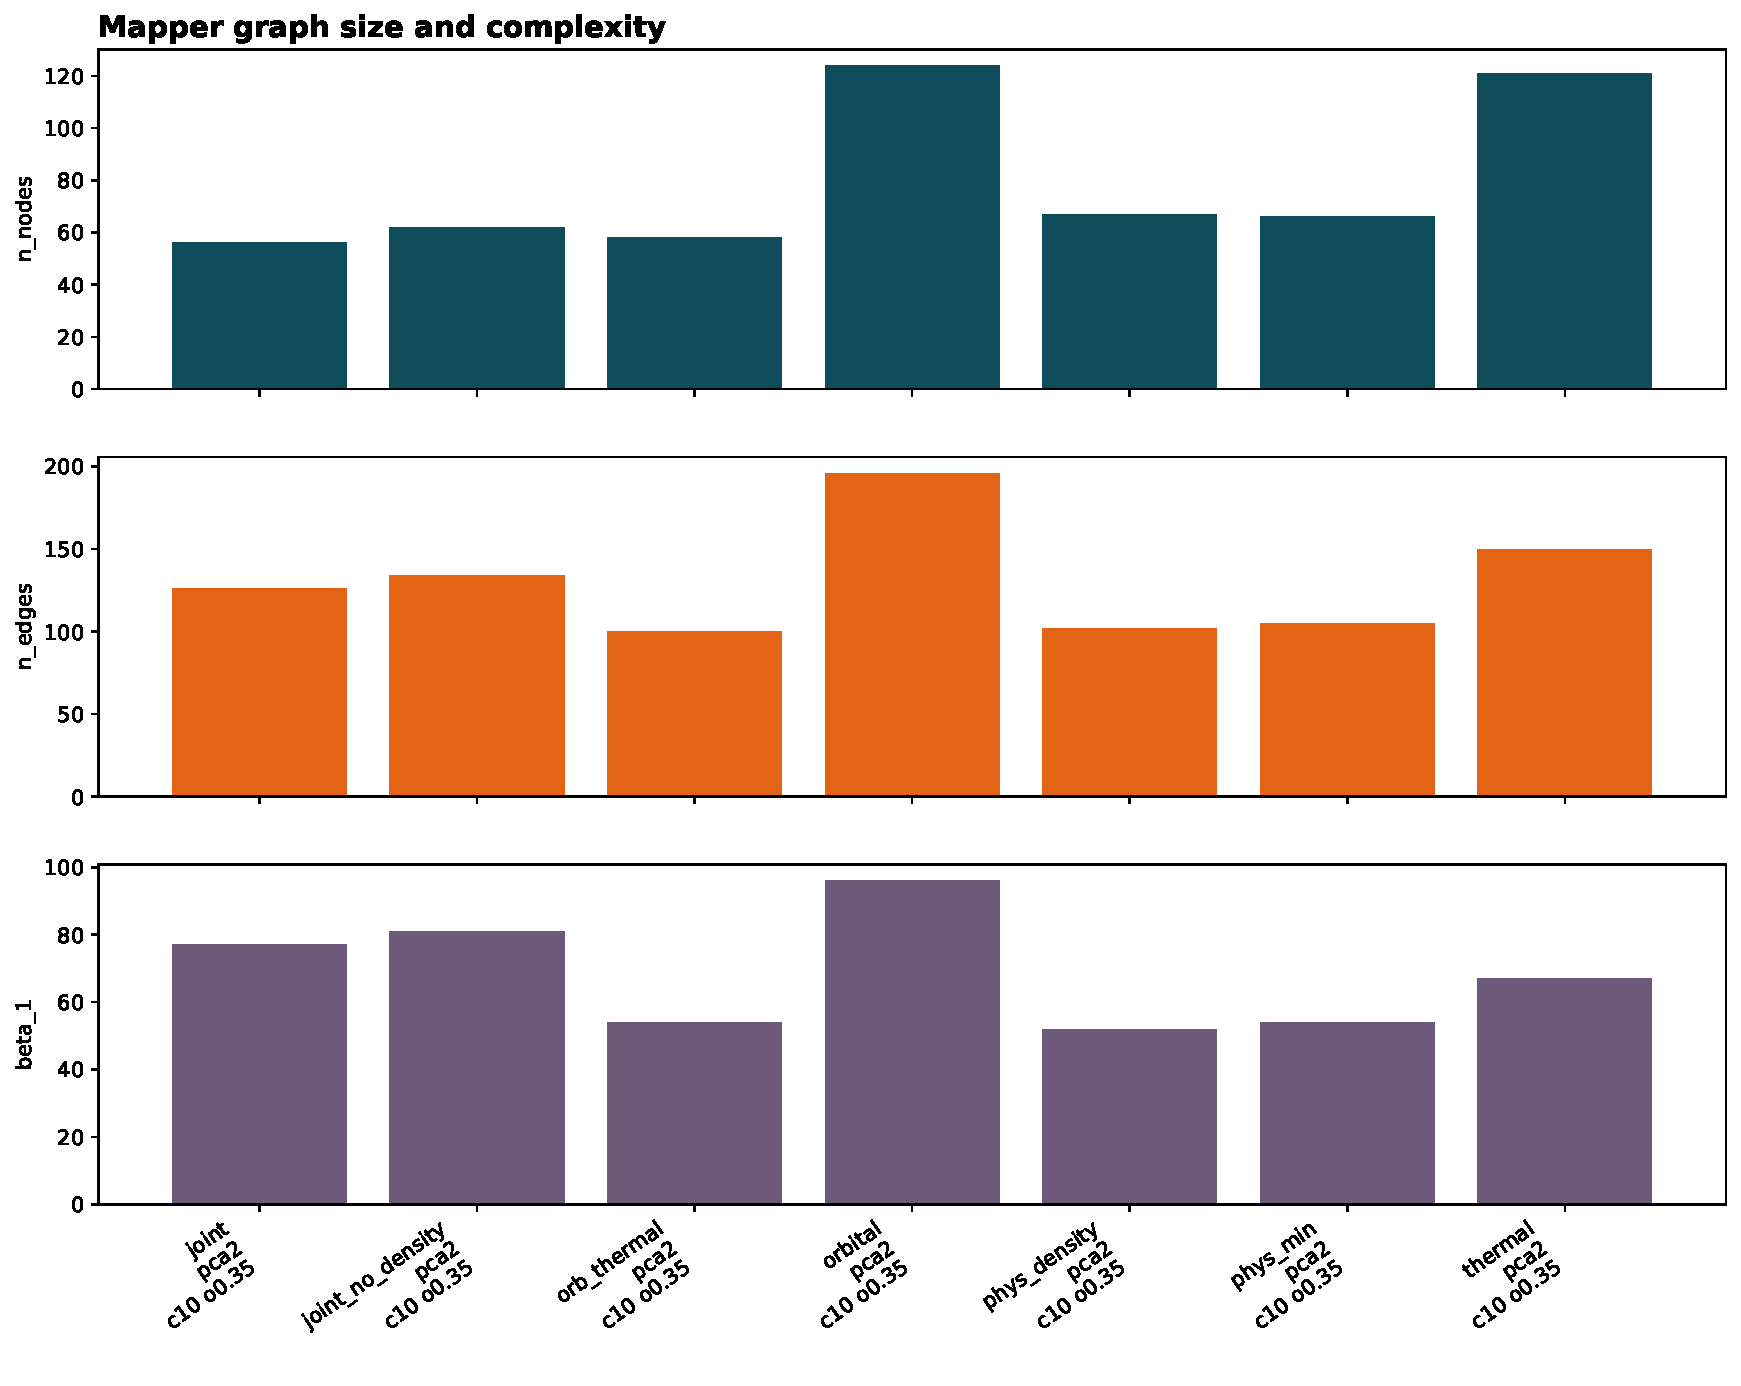
\includegraphics[width=0.95\linewidth]{figures/01_mapper_graph_size_complexity.pdf}\caption{Tamano y complejidad de los grafos Mapper.}\end{figure}\begin{figure}[H]\centering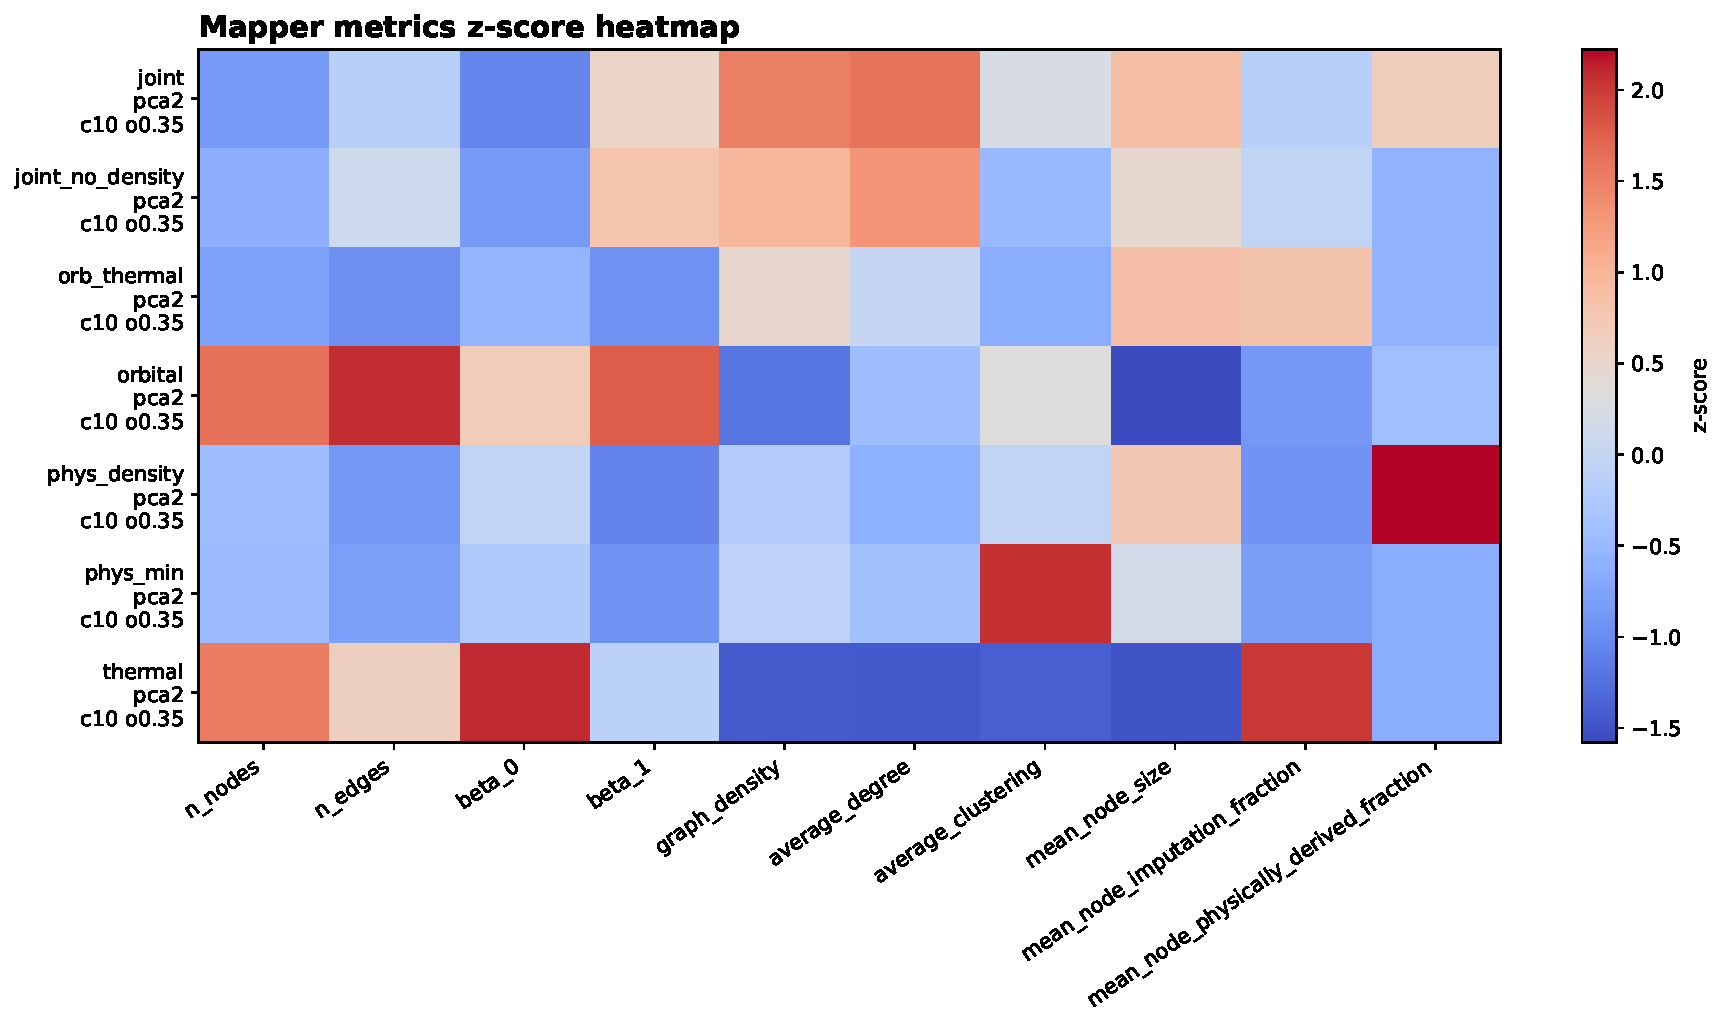
\includegraphics[width=0.95\linewidth]{figures/02_mapper_metrics_zscore_heatmap.pdf}\caption{Heatmap de metricas estandarizadas.}\end{figure}\begin{figure}[H]\centering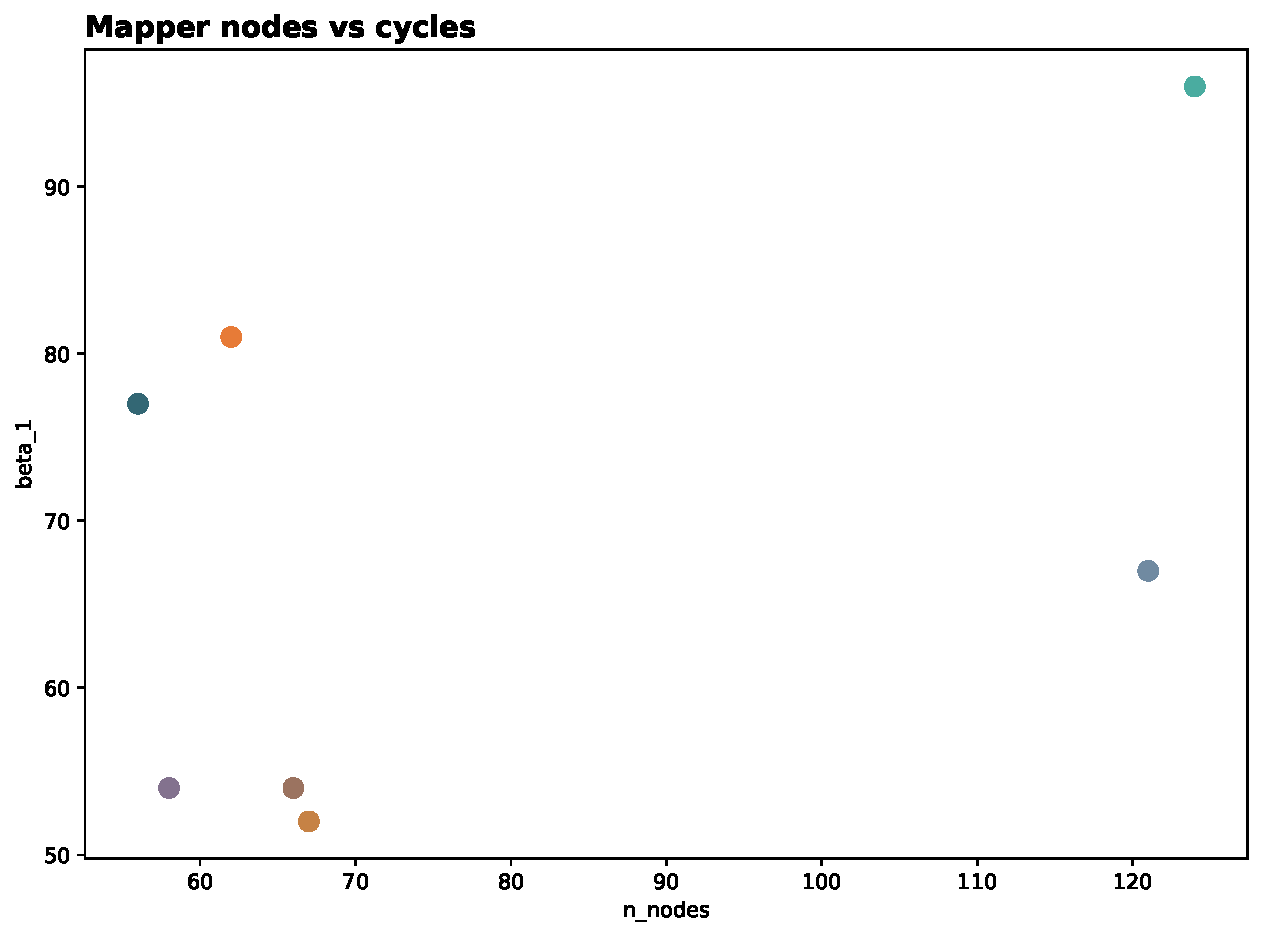
\includegraphics[width=0.75\linewidth]{figures/04_mapper_nodes_vs_cycles.pdf}\caption{Relacion entre numero de nodos y ciclos.}\end{figure}

\section{Sensitivity Analysis}
Adding `pl_dens` reduces the number of independent cycles, suggesting that the derived density feature may simplify or collapse part of the Mapper geometry. No se pudo comparar estabilidad entre lenses. This configuration contains a high average node-level imputation fraction; its topology should be interpreted cautiously. \begin{figure}[H]\centering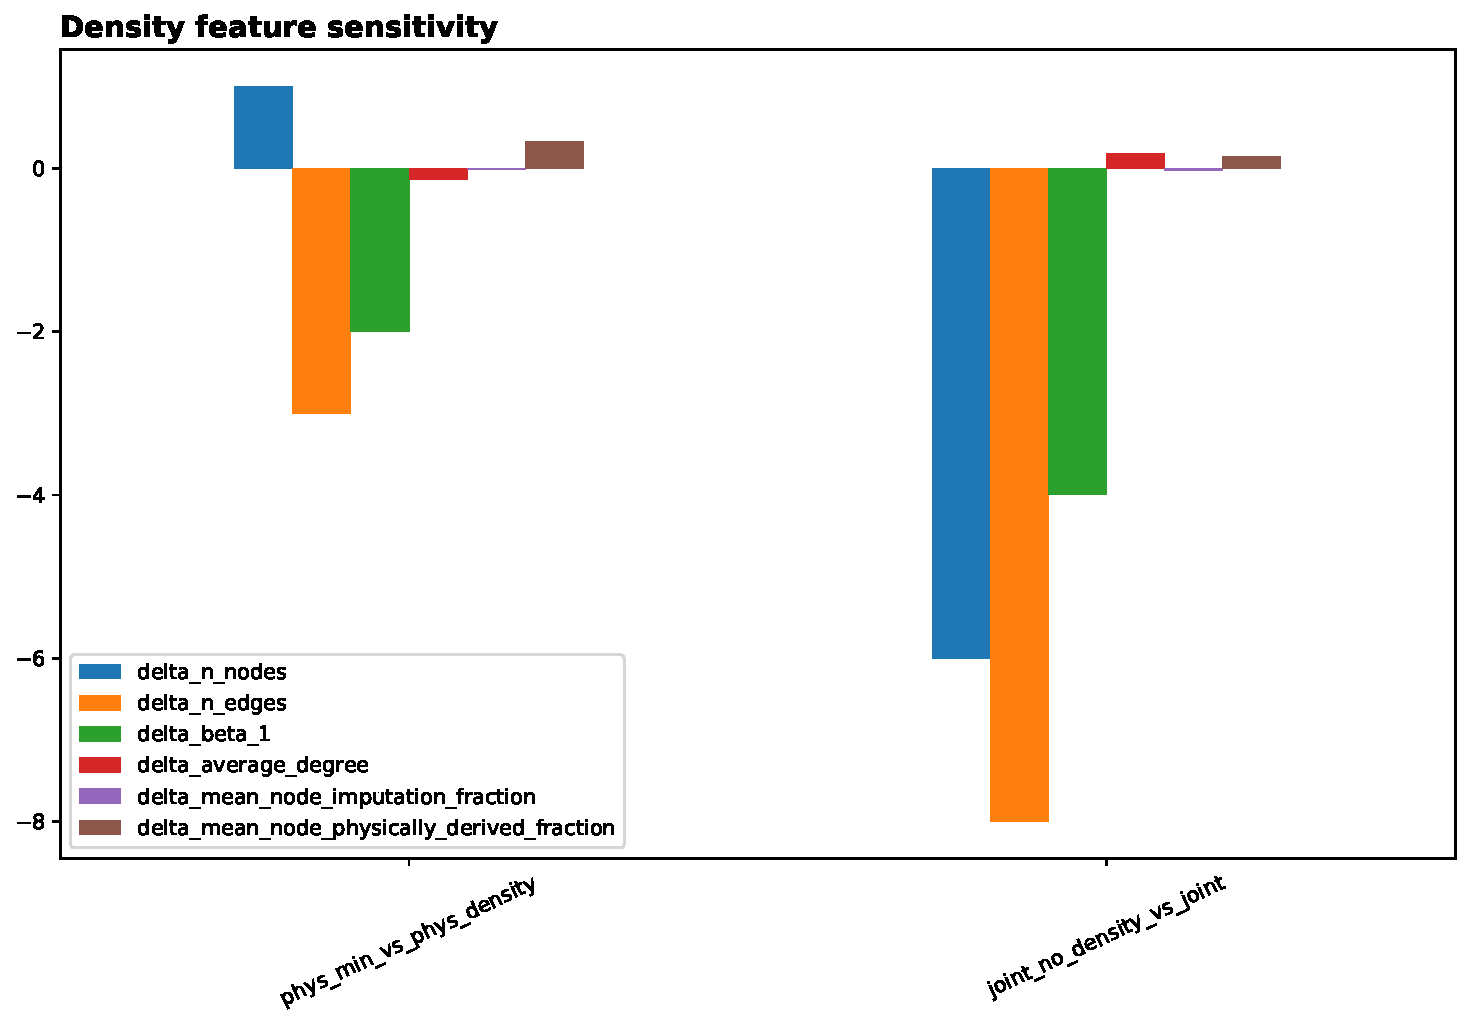
\includegraphics[width=0.9\linewidth]{figures/06_mapper_density_feature_sensitivity.pdf}\caption{Sensibilidad al agregar pl\_dens.}\end{figure}\begin{figure}[H]\centering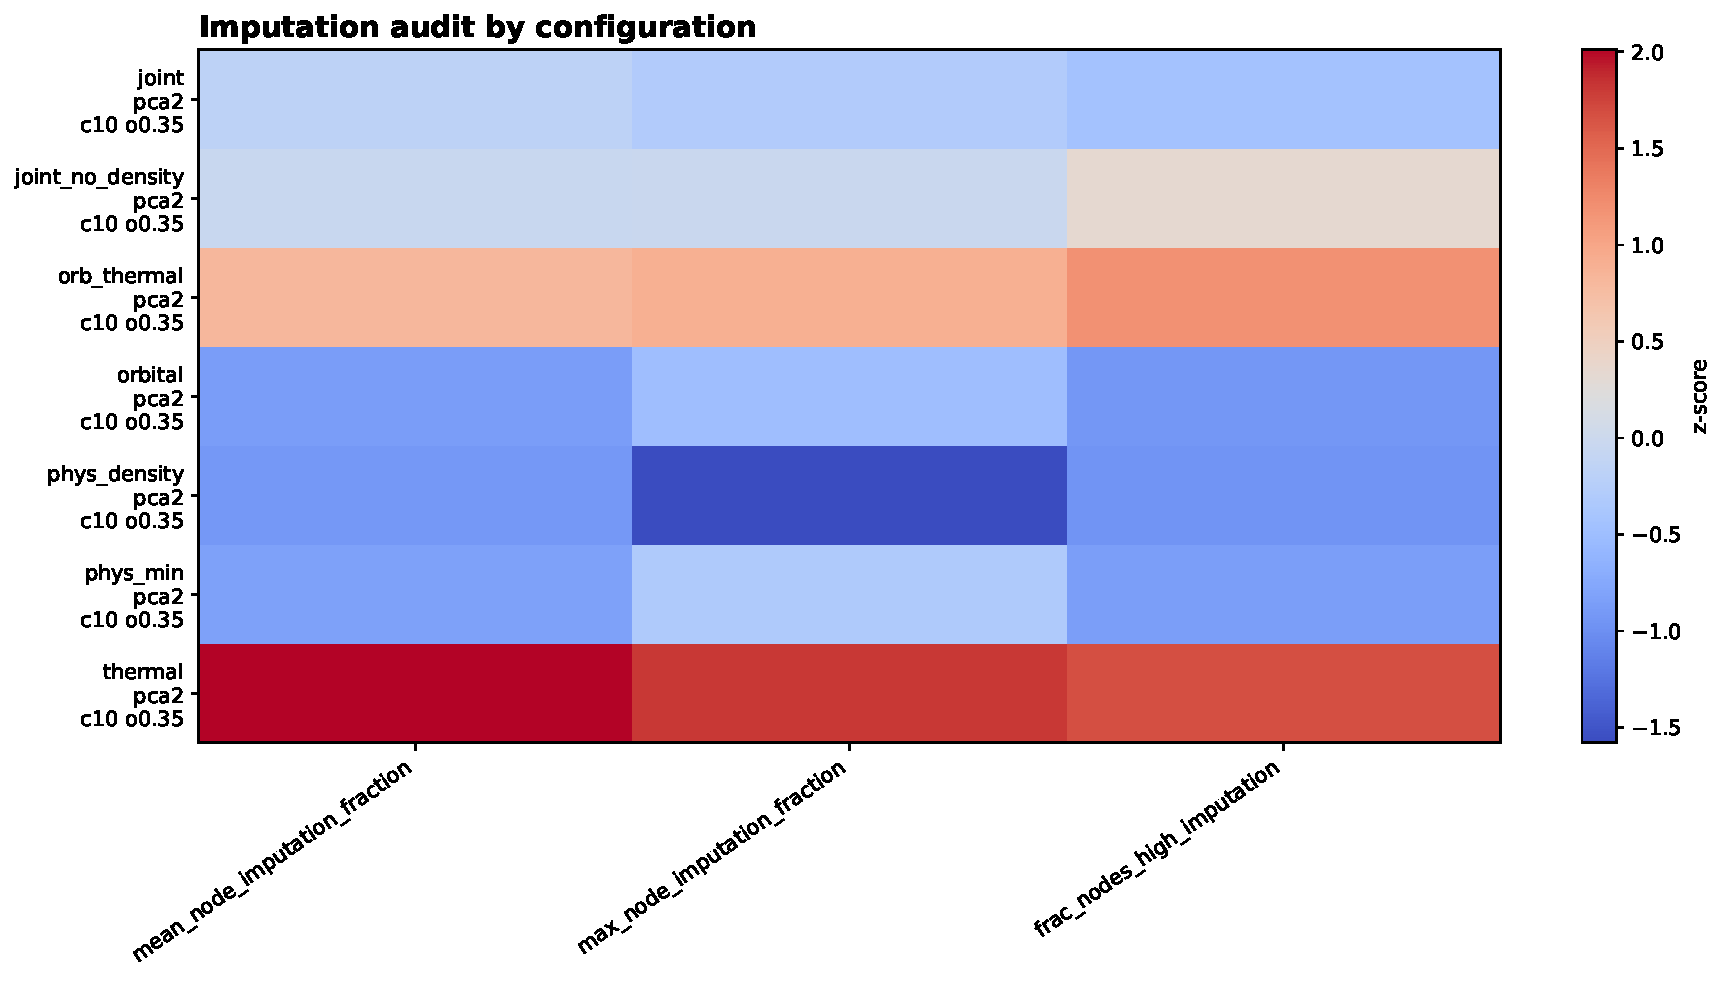
\includegraphics[width=0.9\linewidth]{figures/05_mapper_imputation_audit_by_config.pdf}\caption{Auditoria de imputacion por configuracion.}\end{figure}\begin{figure}[H]\centering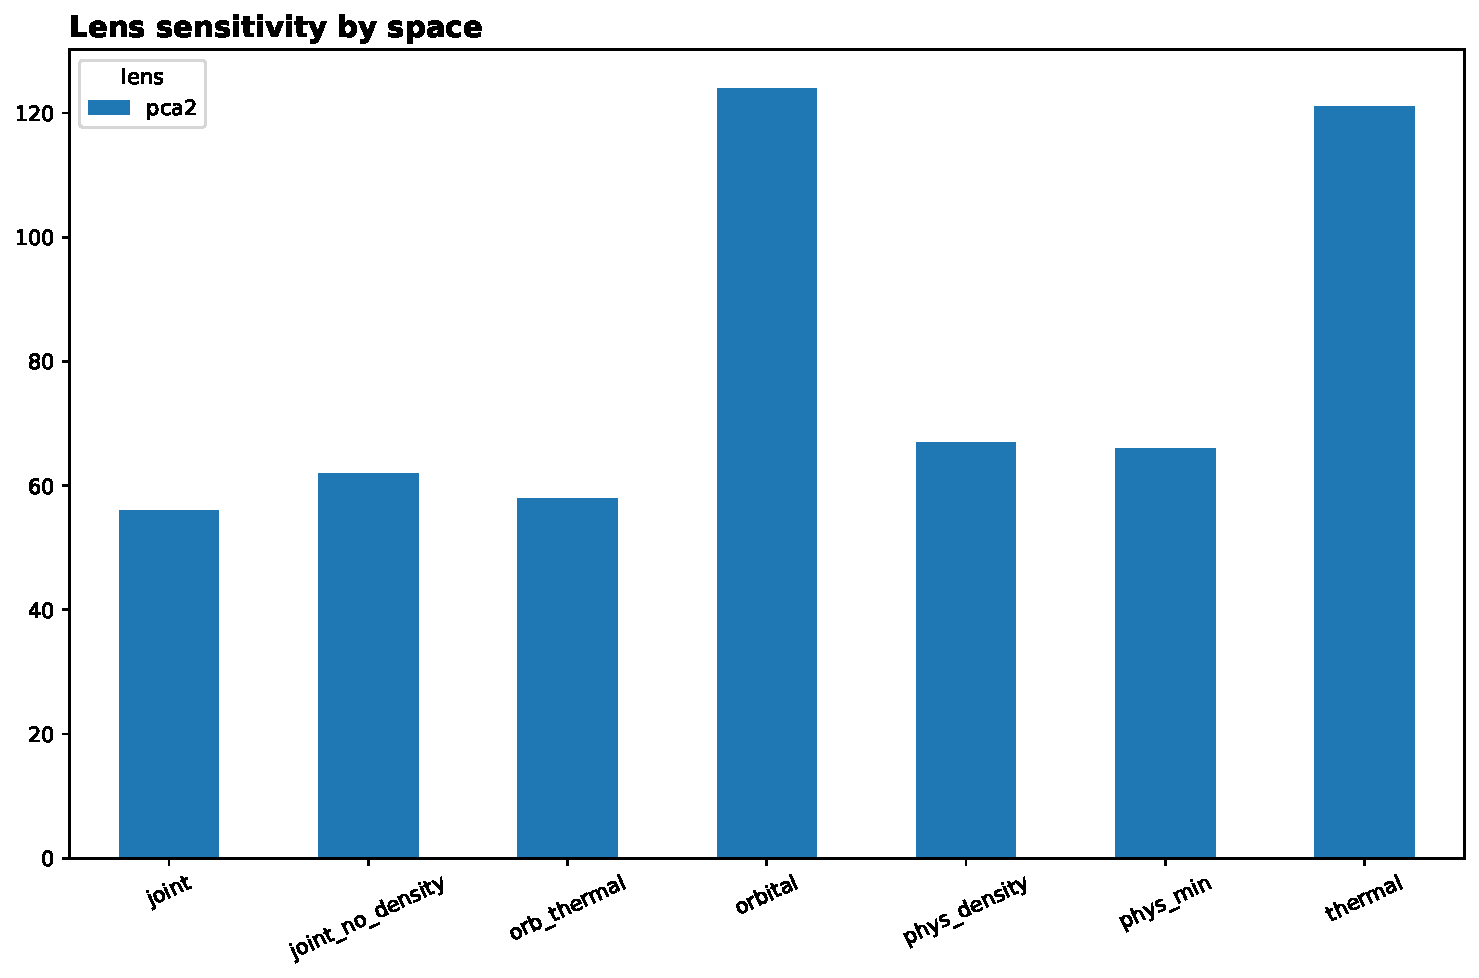
\includegraphics[width=0.9\linewidth]{figures/07_mapper_lens_sensitivity.pdf}\caption{Sensibilidad al lens.}\end{figure}\begin{figure}[H]\centering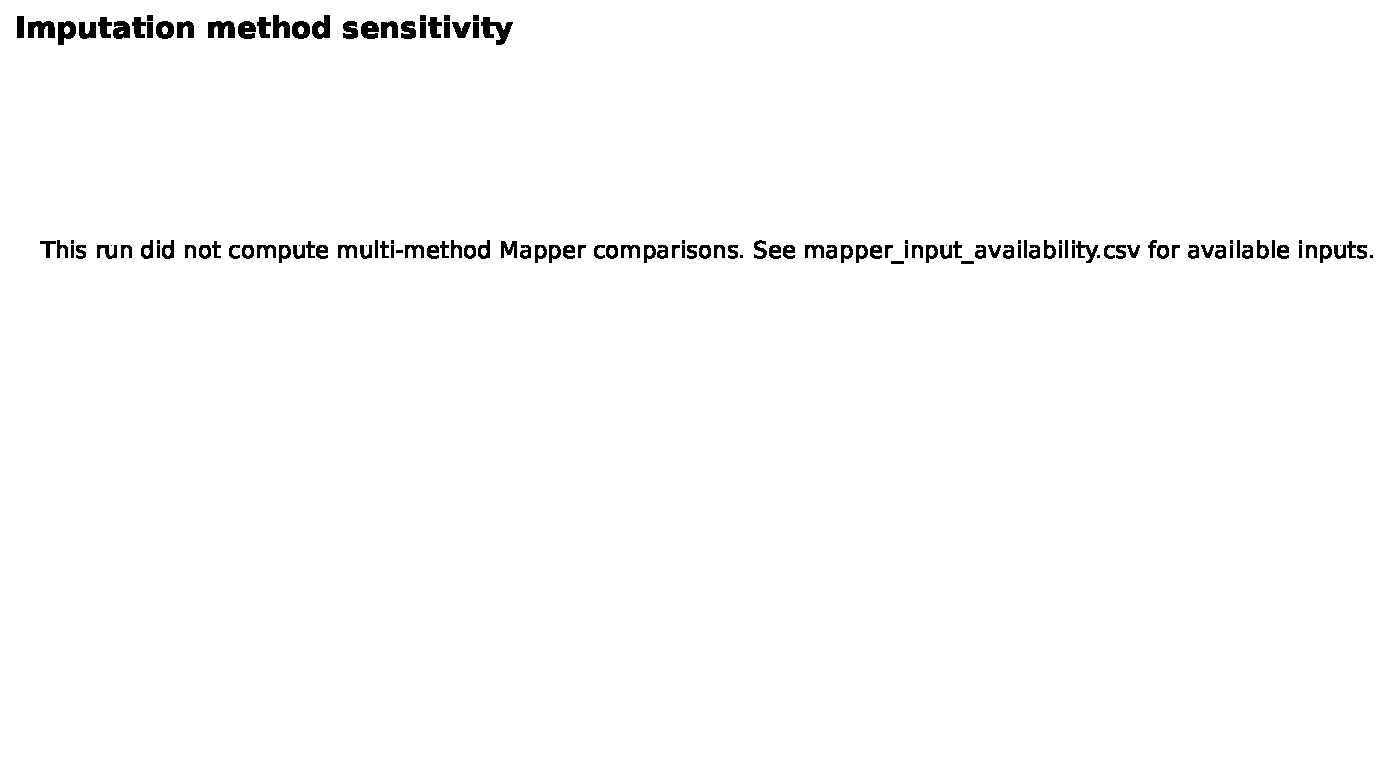
\includegraphics[width=0.9\linewidth]{figures/08_mapper_imputation_method_sensitivity.pdf}\caption{Sensibilidad al metodo de imputacion cuando hay insumos comparables.}\end{figure}

\section{Interpretation}
Mapper muestra estructura topologica inducida por un espacio de variables completado y auditado. Las estructuras con mayor credibilidad son las que persisten entre espacios, lenses y controles de imputacion, y que ademas tienen interpretacion fisica. Las regiones compatibles con rocosos, super-Tierras, sub-Neptunos, gigantes gaseosos o hot Jupiters solo deben enfatizarse si los nodos correspondientes muestran consistencia fisica y baja dependencia de imputacion.

\section{Limitations}
Las limitaciones principales incluyen sesgo observacional por discoverymethod, variables derivadas no independientes, imputacion que no equivale a observacion, dependencia de parametros Mapper, y el hecho de que un beta_1 alto no implica automaticamente estructura fisica. La distancia metric\_zscore\_l2 es una distancia entre vectores de metricas estandarizadas, no una distancia topologica estricta. observed != physically_derived != imputed.

\section{Conclusion}
El pipeline Mapper quedo actualizado para usar iterative por defecto, generar outputs estaticos en outputs/mapper y producir un reporte LaTeX autocontenido. Los siguientes pasos recomendados son estabilidad por bootstrap y revision cientifica de nodos destacados.

\FloatBarrier
\clearpage
\begin{landscape}
\footnotesize
\begin{table}[p]
\centering
\caption{Mapper graph metrics summary.}
\label{tab:mapper_graph_metrics_summary}
\begin{adjustbox}{max width=\linewidth}
\begin{tabular}{llllrrlrrrrrrrrrrrrrrrrrrrrrrrrr}
\toprule
config\_id & input\_method & space & lens & n\_cubes & overlap & clusterer & min\_samples & eps\_percentile & rows\_used & n\_features & mean\_node\_imputation\_fraction & max\_node\_imputation\_fraction & mean\_node\_physically\_derived\_fraction & frac\_nodes\_high\_imputation & frac\_nodes\_high\_derived & config\_has\_density\_feature & n\_nodes & n\_edges & beta\_0 & beta\_1 & graph\_density & average\_degree & average\_clustering & transitivity & n\_isolates & largest\_component\_size & largest\_component\_fraction & mean\_node\_size & median\_node\_size & min\_node\_size & max\_node\_size \\
\midrule
joint\_density\_cubes10\_overlap0p35 & iterative & joint & density & 10 & 0.350 & dbscan & 4 & 90.000 & 6273 & 7 & 0.106 & 0.429 & 0.147 & 0.120 & 0.000 & True & 117 & 260 & 10 & 153 & 0.038 & 4.444 & 0.652 & 0.213 & 4 & 103 & 0.880 & 113.256 & 10.000 & 3 & 1685 \\
joint\_domain\_cubes10\_overlap0p35 & iterative & joint & domain & 10 & 0.350 & dbscan & 4 & 90.000 & 6273 & 7 & 0.121 & 0.571 & 0.139 & 0.125 & 0.000 & True & 64 & 116 & 7 & 59 & 0.058 & 3.625 & 0.445 & 0.333 & 2 & 54 & 0.844 & 209.797 & 8.000 & 3 & 2552 \\
joint\_pca2\_cubes10\_overlap0p35 & iterative & joint & pca2 & 10 & 0.350 & dbscan & 4 & 90.000 & 6273 & 7 & 0.152 & 0.429 & 0.148 & 0.143 & 0.000 & True & 56 & 126 & 7 & 77 & 0.082 & 4.500 & 0.573 & 0.466 & 0 & 40 & 0.714 & 246.054 & 23.000 & 4 & 2384 \\
joint\_no\_density\_density\_cubes10\_overlap0p35 & iterative & joint\_no\_density & density & 10 & 0.350 & dbscan & 4 & 90.000 & 6273 & 6 & 0.142 & 0.500 & 0.005 & 0.257 & 0.000 & False & 109 & 233 & 10 & 134 & 0.040 & 4.275 & 0.675 & 0.266 & 4 & 93 & 0.853 & 122.101 & 7.000 & 3 & 1797 \\
joint\_no\_density\_domain\_cubes10\_overlap0p35 & iterative & joint\_no\_density & domain & 10 & 0.350 & dbscan & 4 & 90.000 & 6273 & 6 & 0.212 & 0.500 & 0.001 & 0.333 & 0.000 & False & 9 & 0 & 9 & 0 & 0.000 & 0.000 & 0.000 & 0.000 & 9 & 1 & 0.111 & 651.333 & 4.000 & 3 & 5825 \\
joint\_no\_density\_pca2\_cubes10\_overlap0p35 & iterative & joint\_no\_density & pca2 & 10 & 0.350 & dbscan & 4 & 90.000 & 6273 & 6 & 0.176 & 0.500 & 0.008 & 0.355 & 0.000 & False & 62 & 134 & 9 & 81 & 0.071 & 4.323 & 0.542 & 0.454 & 3 & 47 & 0.758 & 220.645 & 23.000 & 3 & 2500 \\
orb\_thermal\_density\_cubes10\_overlap0p35 & iterative & orb\_thermal & density & 10 & 0.350 & dbscan & 4 & 90.000 & 6273 & 4 & 0.255 & 0.750 & 0.009 & 0.421 & 0.000 & False & 121 & 246 & 13 & 138 & 0.034 & 4.066 & 0.688 & 0.232 & 6 & 97 & 0.802 & 111.843 & 6.000 & 3 & 2520 \\
orb\_thermal\_domain\_cubes10\_overlap0p35 & iterative & orb\_thermal & domain & 10 & 0.350 & dbscan & 4 & 90.000 & 6273 & 4 & 0.254 & 0.750 & 0.011 & 0.429 & 0.000 & False & 56 & 82 & 12 & 38 & 0.053 & 2.929 & 0.384 & 0.355 & 6 & 40 & 0.714 & 242.607 & 8.000 & 3 & 2762 \\
orb\_thermal\_pca2\_cubes10\_overlap0p35 & iterative & orb\_thermal & pca2 & 10 & 0.350 & dbscan & 4 & 90.000 & 6273 & 4 & 0.347 & 0.750 & 0.009 & 0.586 & 0.000 & False & 58 & 100 & 12 & 54 & 0.060 & 3.448 & 0.536 & 0.476 & 4 & 36 & 0.621 & 244.793 & 6.500 & 3 & 2847 \\
orbital\_density\_cubes10\_overlap0p35 & iterative & orbital & density & 10 & 0.350 & dbscan & 4 & 90.000 & 6273 & 2 & 0.030 & 0.385 & 0.028 & 0.022 & 0.000 & False & 178 & 297 & 25 & 144 & 0.019 & 3.337 & 0.543 & 0.135 & 6 & 117 & 0.657 & 76.090 & 7.000 & 3 & 2389 \\
orbital\_domain\_cubes10\_overlap0p35 & iterative & orbital & domain & 10 & 0.350 & dbscan & 4 & 90.000 & 6273 & 2 & 0.034 & 0.375 & 0.030 & 0.013 & 0.000 & False & 77 & 94 & 25 & 42 & 0.032 & 2.442 & 0.665 & 0.862 & 4 & 13 & 0.169 & 189.896 & 6.000 & 3 & 3206 \\
orbital\_pca2\_cubes10\_overlap0p35 & iterative & orbital & pca2 & 10 & 0.350 & dbscan & 4 & 90.000 & 6273 & 2 & 0.011 & 0.375 & 0.028 & 0.008 & 0.000 & False & 124 & 196 & 24 & 96 & 0.026 & 3.161 & 0.577 & 0.215 & 4 & 62 & 0.500 & 91.573 & 6.000 & 3 & 3316 \\
\bottomrule
\end{tabular}
\end{adjustbox}
\end{table}

\input{tables/mapper_space_comparison.tex}
\begin{table}
\caption{Density feature sensitivity.}
\label{tab:mapper_density_sensitivity}
\begin{tabular}{lllrrrrrr}
\toprule
comparison & without\_density & with\_density & delta\_n\_nodes & delta\_n\_edges & delta\_beta\_1 & delta\_average\_degree & delta\_mean\_node\_imputation\_fraction & delta\_mean\_node\_physically\_derived\_fraction \\
\midrule
phys\_min\_vs\_phys\_density & phys\_min & phys\_density & 1.000 & -3.000 & -2.000 & -0.137 & -0.016 & 0.332 \\
joint\_no\_density\_vs\_joint & joint\_no\_density & joint & -6.000 & -8.000 & -4.000 & 0.177 & -0.024 & 0.140 \\
\bottomrule
\end{tabular}
\end{table}

\begin{table}[p]
\centering
\caption{Lens sensitivity summary.}
\label{tab:mapper_lens_sensitivity}
\begin{adjustbox}{max width=\linewidth}
\begin{tabular}{llllrrlrrrrrrrrrrrrrrrrrrrrrrrrr}
\toprule
config\_id & input\_method & space & lens & n\_cubes & overlap & clusterer & min\_samples & eps\_percentile & rows\_used & n\_features & mean\_node\_imputation\_fraction & max\_node\_imputation\_fraction & mean\_node\_physically\_derived\_fraction & frac\_nodes\_high\_imputation & frac\_nodes\_high\_derived & config\_has\_density\_feature & n\_nodes & n\_edges & beta\_0 & beta\_1 & graph\_density & average\_degree & average\_clustering & transitivity & n\_isolates & largest\_component\_size & largest\_component\_fraction & mean\_node\_size & median\_node\_size & min\_node\_size & max\_node\_size \\
\midrule
joint\_density\_cubes10\_overlap0p35 & iterative & joint & density & 10 & 0.350 & dbscan & 4 & 90.000 & 6273 & 7 & 0.106 & 0.429 & 0.147 & 0.120 & 0.000 & True & 117 & 260 & 10 & 153 & 0.038 & 4.444 & 0.652 & 0.213 & 4 & 103 & 0.880 & 113.256 & 10.000 & 3 & 1685 \\
joint\_domain\_cubes10\_overlap0p35 & iterative & joint & domain & 10 & 0.350 & dbscan & 4 & 90.000 & 6273 & 7 & 0.121 & 0.571 & 0.139 & 0.125 & 0.000 & True & 64 & 116 & 7 & 59 & 0.058 & 3.625 & 0.445 & 0.333 & 2 & 54 & 0.844 & 209.797 & 8.000 & 3 & 2552 \\
joint\_pca2\_cubes10\_overlap0p35 & iterative & joint & pca2 & 10 & 0.350 & dbscan & 4 & 90.000 & 6273 & 7 & 0.152 & 0.429 & 0.148 & 0.143 & 0.000 & True & 56 & 126 & 7 & 77 & 0.082 & 4.500 & 0.573 & 0.466 & 0 & 40 & 0.714 & 246.054 & 23.000 & 4 & 2384 \\
joint\_no\_density\_density\_cubes10\_overlap0p35 & iterative & joint\_no\_density & density & 10 & 0.350 & dbscan & 4 & 90.000 & 6273 & 6 & 0.142 & 0.500 & 0.005 & 0.257 & 0.000 & False & 109 & 233 & 10 & 134 & 0.040 & 4.275 & 0.675 & 0.266 & 4 & 93 & 0.853 & 122.101 & 7.000 & 3 & 1797 \\
joint\_no\_density\_domain\_cubes10\_overlap0p35 & iterative & joint\_no\_density & domain & 10 & 0.350 & dbscan & 4 & 90.000 & 6273 & 6 & 0.212 & 0.500 & 0.001 & 0.333 & 0.000 & False & 9 & 0 & 9 & 0 & 0.000 & 0.000 & 0.000 & 0.000 & 9 & 1 & 0.111 & 651.333 & 4.000 & 3 & 5825 \\
joint\_no\_density\_pca2\_cubes10\_overlap0p35 & iterative & joint\_no\_density & pca2 & 10 & 0.350 & dbscan & 4 & 90.000 & 6273 & 6 & 0.176 & 0.500 & 0.008 & 0.355 & 0.000 & False & 62 & 134 & 9 & 81 & 0.071 & 4.323 & 0.542 & 0.454 & 3 & 47 & 0.758 & 220.645 & 23.000 & 3 & 2500 \\
orb\_thermal\_density\_cubes10\_overlap0p35 & iterative & orb\_thermal & density & 10 & 0.350 & dbscan & 4 & 90.000 & 6273 & 4 & 0.255 & 0.750 & 0.009 & 0.421 & 0.000 & False & 121 & 246 & 13 & 138 & 0.034 & 4.066 & 0.688 & 0.232 & 6 & 97 & 0.802 & 111.843 & 6.000 & 3 & 2520 \\
orb\_thermal\_domain\_cubes10\_overlap0p35 & iterative & orb\_thermal & domain & 10 & 0.350 & dbscan & 4 & 90.000 & 6273 & 4 & 0.254 & 0.750 & 0.011 & 0.429 & 0.000 & False & 56 & 82 & 12 & 38 & 0.053 & 2.929 & 0.384 & 0.355 & 6 & 40 & 0.714 & 242.607 & 8.000 & 3 & 2762 \\
orb\_thermal\_pca2\_cubes10\_overlap0p35 & iterative & orb\_thermal & pca2 & 10 & 0.350 & dbscan & 4 & 90.000 & 6273 & 4 & 0.347 & 0.750 & 0.009 & 0.586 & 0.000 & False & 58 & 100 & 12 & 54 & 0.060 & 3.448 & 0.536 & 0.476 & 4 & 36 & 0.621 & 244.793 & 6.500 & 3 & 2847 \\
orbital\_density\_cubes10\_overlap0p35 & iterative & orbital & density & 10 & 0.350 & dbscan & 4 & 90.000 & 6273 & 2 & 0.030 & 0.385 & 0.028 & 0.022 & 0.000 & False & 178 & 297 & 25 & 144 & 0.019 & 3.337 & 0.543 & 0.135 & 6 & 117 & 0.657 & 76.090 & 7.000 & 3 & 2389 \\
orbital\_domain\_cubes10\_overlap0p35 & iterative & orbital & domain & 10 & 0.350 & dbscan & 4 & 90.000 & 6273 & 2 & 0.034 & 0.375 & 0.030 & 0.013 & 0.000 & False & 77 & 94 & 25 & 42 & 0.032 & 2.442 & 0.665 & 0.862 & 4 & 13 & 0.169 & 189.896 & 6.000 & 3 & 3206 \\
orbital\_pca2\_cubes10\_overlap0p35 & iterative & orbital & pca2 & 10 & 0.350 & dbscan & 4 & 90.000 & 6273 & 2 & 0.011 & 0.375 & 0.028 & 0.008 & 0.000 & False & 124 & 196 & 24 & 96 & 0.026 & 3.161 & 0.577 & 0.215 & 4 & 62 & 0.500 & 91.573 & 6.000 & 3 & 3316 \\
phys\_density\_density\_cubes10\_overlap0p35 & iterative & phys\_density & density & 10 & 0.350 & dbscan & 4 & 90.000 & 6273 & 3 & 0.002 & 0.084 & 0.332 & 0.000 & 0.987 & True & 78 & 109 & 21 & 52 & 0.036 & 2.795 & 0.444 & 0.451 & 6 & 39 & 0.500 & 164.974 & 18.000 & 4 & 2431 \\
phys\_density\_domain\_cubes10\_overlap0p35 & iterative & phys\_density & domain & 10 & 0.350 & dbscan & 4 & 90.000 & 6273 & 3 & 0.010 & 0.527 & 0.328 & 0.013 & 0.975 & True & 80 & 132 & 16 & 68 & 0.042 & 3.300 & 0.622 & 0.482 & 4 & 44 & 0.550 & 172.325 & 6.000 & 4 & 2563 \\
phys\_density\_pca2\_cubes10\_overlap0p35 & iterative & phys\_density & pca2 & 10 & 0.350 & dbscan & 4 & 90.000 & 6273 & 3 & 0.002 & 0.079 & 0.332 & 0.000 & 0.985 & True & 67 & 102 & 17 & 52 & 0.046 & 3.045 & 0.561 & 0.529 & 7 & 33 & 0.493 & 238.388 & 6.000 & 3 & 3023 \\
phys\_min\_density\_cubes10\_overlap0p35 & iterative & phys\_min & density & 10 & 0.350 & dbscan & 4 & 90.000 & 6273 & 2 & 0.010 & 0.417 & 0.000 & 0.010 & 0.000 & False & 97 & 152 & 20 & 75 & 0.033 & 3.134 & 0.521 & 0.430 & 4 & 53 & 0.546 & 138.000 & 9.000 & 3 & 1735 \\
phys\_min\_domain\_cubes10\_overlap0p35 & iterative & phys\_min & domain & 10 & 0.350 & dbscan & 4 & 90.000 & 6273 & 2 & 0.010 & 0.269 & 0.000 & 0.000 & 0.000 & False & 76 & 125 & 15 & 64 & 0.044 & 3.289 & 0.745 & 0.603 & 2 & 34 & 0.447 & 173.513 & 7.000 & 3 & 2380 \\
phys\_min\_pca2\_cubes10\_overlap0p35 & iterative & phys\_min & pca2 & 10 & 0.350 & dbscan & 4 & 90.000 & 6273 & 2 & 0.017 & 0.421 & 0.000 & 0.030 & 0.000 & False & 66 & 105 & 15 & 54 & 0.049 & 3.182 & 0.649 & 0.579 & 6 & 33 & 0.500 & 202.545 & 7.000 & 3 & 2323 \\
\bottomrule
\end{tabular}
\end{adjustbox}
\end{table}

\begin{table}[p]
\centering
\caption{Imputation audit summary.}
\label{tab:mapper_imputation_audit_summary}
\begin{adjustbox}{max width=\linewidth}
\begin{tabular}{lrrr}
\toprule
config\_id & mean\_node\_imputation\_fraction & max\_node\_imputation\_fraction & frac\_nodes\_high\_imputation \\
\midrule
joint\_density\_cubes10\_overlap0p35 & 0.106 & 0.429 & 0.120 \\
joint\_domain\_cubes10\_overlap0p35 & 0.121 & 0.571 & 0.125 \\
joint\_pca2\_cubes10\_overlap0p35 & 0.152 & 0.429 & 0.143 \\
joint\_no\_density\_density\_cubes10\_overlap0p35 & 0.142 & 0.500 & 0.257 \\
joint\_no\_density\_domain\_cubes10\_overlap0p35 & 0.212 & 0.500 & 0.333 \\
joint\_no\_density\_pca2\_cubes10\_overlap0p35 & 0.176 & 0.500 & 0.355 \\
orb\_thermal\_density\_cubes10\_overlap0p35 & 0.255 & 0.750 & 0.421 \\
orb\_thermal\_domain\_cubes10\_overlap0p35 & 0.254 & 0.750 & 0.429 \\
orb\_thermal\_pca2\_cubes10\_overlap0p35 & 0.347 & 0.750 & 0.586 \\
orbital\_density\_cubes10\_overlap0p35 & 0.030 & 0.385 & 0.022 \\
orbital\_domain\_cubes10\_overlap0p35 & 0.034 & 0.375 & 0.013 \\
orbital\_pca2\_cubes10\_overlap0p35 & 0.011 & 0.375 & 0.008 \\
phys\_density\_density\_cubes10\_overlap0p35 & 0.002 & 0.084 & 0.000 \\
phys\_density\_domain\_cubes10\_overlap0p35 & 0.010 & 0.527 & 0.013 \\
phys\_density\_pca2\_cubes10\_overlap0p35 & 0.002 & 0.079 & 0.000 \\
phys\_min\_density\_cubes10\_overlap0p35 & 0.010 & 0.417 & 0.010 \\
phys\_min\_domain\_cubes10\_overlap0p35 & 0.010 & 0.269 & 0.000 \\
phys\_min\_pca2\_cubes10\_overlap0p35 & 0.017 & 0.421 & 0.030 \\
thermal\_density\_cubes10\_overlap0p35 & 0.472 & 1.000 & 0.541 \\
thermal\_domain\_cubes10\_overlap0p35 & 0.527 & 1.000 & 0.621 \\
thermal\_pca2\_cubes10\_overlap0p35 & 0.588 & 1.000 & 0.719 \\
\bottomrule
\end{tabular}
\end{adjustbox}
\end{table}

\end{landscape}
\end{document}
